%%
%% ****** Generated 24.03.23 by LJM TeX-constructor******
%%
\documentclass[
11pt,%
tightenlines,%
twoside,%
onecolumn,%
nofloats,%
nobibnotes,%
nofootinbib,%
superscriptaddress,%
noshowpacs,%
centertags]%
{revtex4}
\usepackage{ljm}



%\setcounter{page}{3}

\begin{document}
\titlerunning{Influence of weight coefficients on the solution of the inverse problem} % for running heads
\authorrunning{Kosyakov} % for running heads
%\authorrunning{First-Author, Second-Author} % for running heads

\title{Investigation of the Influence of Weight Coefficients in Solving
the Problem of Permeability Identification for an Oil Field}
% Splitting into lines is performed by the command \\
% The title is written in accordance with the rules of capitalization.

\author{\firstname{V. P.}~\surname{Kosyakov}}
\email[E-mail: ]{lik.24@yandex.ru} \affiliation{Tyumen Branch of
Khristianovich Institute of Theoretical and Applied  Mechanics SB
RAS, Taymirskaya ul. 74, 625026, Tyumen, Russia}


%\noaffiliation % If the author does not specify a place of work.

%\firstcollaboration{(Submitted by ) } % Add if you know submitter.
%\lastcollaboration{ }

\firstcollaboration{(Submitted by D. A. Gubaidullin)} % Add if you know submitter.
%\lastcollaboration{ }

\received{March 2, 2023; revised March 24, 2023; accepted March 30,
2023}

\begin{abstract} % You shouldn't use formulas and citations in the abstract.
Solution of the inverse problem is one of important steps at the process of the oil field development modelling. As a rule, the solution includes the selection of model parameters for the best match to the development history data. To solve the inverse problem, heterogeneous original data are used. The degree of influence on the result of the solution is determined by weight coefficients of the data. In addition, the purpose of the modelling is not only to repeat the development performance for the "historical period", but also to obtain a reliable forecast of the behaviour of the modelled object in the future. In this paper, on the example of solving the parametic identification problem of the reservoir permeability for modelling the oil field development, there is investigated the study of the influence of the choice of weight coefficients on the accuracy of the model matching and its forecasting characteristics. It
is shown that the correct choice of weight coefficients makes it
possible to obtain a model with the best forecasting properties. To
assess the accuracy of the model and select the option of its
history matching, it is recommended to use additional metrics other
than the objective function.
\end{abstract}
\subclass{76S05,90C31} % Enter 2010 Mathematics Subject Classification.
\keywords{inverse problem, parametric identification, hydrodynamic simulation, flow through porous medium, metric} % Include keywords separeted by comma.

\maketitle

% Text of article starts here.



\section{INTRODUCTION}
At the present time, the creation of digital twins of different objects and physical processes, which, as a rule, are based on mathematical models, has become widespread. For the successful use
of such models in practice, a necessary condition is the
reproduction of the actual behavior of the studying object.To satisfy
this requirement for numerical models, the history matching
procedure is performed, which is a solution of an inverse problem in
order to select some model parameters, as well as initial and/or
boundary conditions, if they are not known with sufficient accuracy.

In relation to the problems of fluids flow in porous media, underground
hydrodynamics, and oil field development, the problem of
restoring reservoir permeability is an actual task. Data on the real value of reservoir permeability can be obtained only by drilling wells. The obtained values characerize only a small part of the reservoir - near-wellbore zone. The value of permeability in the interwell space is an estimation. The value
of permeability is one of the important parameters characterizing
the potential and process of oil field development. Therefore, the
problem of restoring or refining the reservoir permeability is an important and actual task. When using a hydrodynamic model and known actual values of the
main development indicators for the historical period (liquid, oil
extraction, water injection, reservoir and bottomhole pressures,
etc.), it becomes possible to obtain a solution to the inverse
problem. The solution is to find such a reservoir permeability, using which the calculated values of the development performance satisfy the actual data with sufficient accuracy.

This paper presents a study of the dependence of the history
matching and forecasting characteristics of the model on the degree
of confidence in the original data of various types. The papers
\cite{mus} and \cite{kos} demonstrated an indirect dependence of the
forecast accuracy on the accuracy of the history matching. On the example of the problem of parametric identification
of a fluid flow model for an oil field in a two-phase formulation,
the importance of using the all available data is shown.
The forecasted value is reservoir pressure, which characterizes
the energy potential of of the development reservoir and water flow 
rates at wells.

\section{Mathematical Model}
A 2D incompressible so called "coloured liquid" model of two-phase flow \cite{bas} was used to solve the problem. The use of a "coloured liquid" model assumes: the same viscosity of fluids equal to $\mu$, directly proportional dependence of the relative phase permeability on the saturation of the corresponding phase, the absence of saturation effect on pressure, capillary forces are not taken into account, the pressure of the phases is taken equal. The fluids flow in porous media
equations can be written as follows
\begin{equation} \label{fil}
\triangledown \cdot \left[\frac{k}{\mu}\triangledown P \right] = \delta_{l}(x,y),
\end{equation}
\begin{equation} \label{fil2}
\frac{\phi\partial S_w}{\partial t} = \triangledown\cdot \left[\frac{kk_{rw}}{\mu}\triangledown P \right] +\delta_w(x,y),
\end{equation}
\begin{equation} \label{bc}
\delta_{i}(x,y)  = \left\{\begin{array}{crl}
0, \;\mbox{if}\;(x,y) \notin\ \Gamma_{in}\cup\Gamma_{out},\\
q_{i\:k}, \;\mbox{if}\;(x,y) \in \Gamma_{in},\\
q_{i\:aq}, \;\mbox{if}\;(x,y) \in \Gamma_{out},
\end{array}\right. \quad i = l,w.
\end{equation}
Closing ratios:
\begin{equation} \label{kr}
 S_w + S_o = 1;\quad
    k_{rw} = S_w, \quad k_{ro} = 1 - S_w; \quad P = P_0,\quad S_w = S_{w0}\mbox{,\quad \mbox{if} $t=0$},
\end{equation}
where $k$ is permeability, $P$ is reservoir pressure, $\phi$ is
porosity, $S$ is saturation, subscript $i$ denotes $l$ -- liquid
(water and oil), $w$ is water, or $k_{r}$ is relative phase
permeability, $q_k$ is fluid flow rate in $k$th well, $\Gamma_{in}$
is set of coordinates of sources/drain (wells), $\Gamma_{out}$ is
outer boundary, $P_0$ is reservoir pressure and $S_{w0}$ is water
saturation at the initial time $t=0$, $q_{aq}$ is specific fluid flow rate through the outer boundary, which can be written as:
\begin{equation*} \label{qaq}
q_{i\:aq} = \lambda \frac{kk_{ri}}{\mu}(P_{a} - P|_{\Gamma_{out}}),
\end{equation*}
where $P_a$ is on the aquifer ($P_a = P_0$), $\lambda$ is
aquifer productivity factor. It is assumed that the water saturation
of the aquifer is $S_{a\:w} = 1$. The goal of the inverse problem is to find the reservior permeability  $k = k(x,y)$ at which the calculated values of reservoir pressure and water flow rate on the wells will satisfactorily coincide with the initial values.
The inverse problem is solved in an optimization
formulation, which consists in minimizing the objective function $J$.
The objective function can be written as a sum of terms, each of which
is the product of a function characterizing the deviation of the
calculated values from the control values and a weighting
coefficient for the corresponding type of variable. The mean square
error (MSE) was chosen as a deviation measure
\begin{equation} \label{mse}
J=w_p\frac{1}{N}\sum_{i=1}^N{\left(p_c^i-p_f^i\right)^2}+
w_{q_w}\frac{1}{M}\sum_{i=1}^M{\left(q_{w\:c}^i-q_{w\:f}^i\right)^2},
\end{equation}
where $p_c^i$ is the calculated value of reservoir pressure, $p_f^i$
is the actual value, $i$ is the measurement number, $N$ is the
number of reservoir pressure measurements, $q_{w\:c}^i$ and $
q_{w\:f}^i$ are calculated and actual value of water flow in wells,
respectively, the subscript $f$ means actual values (fact), and $c$
-- calculated (calculated), $M$ is number of flow measurements well
water, $w_p$ and $w_{q_w}$ are weight coefficients taking into
account the degree of influence of various parameters (dimension,
data quality, etc.). The arguments of the term of the objective
function responsible for pressure are the actual (measured) and
calculated values of the reservoir pressure at the well locations at
the given time points. The calculated values, in turn, depend on the
model parameters $u$. The solution is found using the gradient
optimization algorithm and consists in determining the set of model
parameters corresponding to the minimum $J$ and satisfying the
constraints in the form of inequalities
$
u_{min}\leq\ \boldsymbol{u}\leq u_{max},
$
$u_{min}$ and $u_{max}$ are minimum and maximum value for 
parameter.

The optimization problem is solved when each component of the gradient of the objective function tends to 0, which can be written as:
\begin{equation}\label{grad}
\frac{\partial J}{\partial u_k} = 2w_p\frac{1}{N}\sum_{i=1}^N
({p_c^i-p_f^i}) \frac{\partial p_c^i}{\partial
u_k}+2w_{q_w}\frac{1}{M}\sum_{i=1}^M{\left(q_{w\:c}^i-q_{w\:f}^i\right)}\frac{\partial
q_{w\:c}^i}{\partial u_k}.
\end{equation}
To solve the optimization problem, it is necessary that each
component  of the objective function gradient tends to 0, which can
be written as
\begin{equation} \label{rp}
     \frac{\partial J}{\partial u_k} \rightarrow 0.
\end{equation}
The solution of the inverse problem (\ref{rp}) is found  numerically
by the iterative method. At each iteration, the direct problem
(\ref{fil})--(\ref{bc}) is numerically solved and the derivatives of
the objective function are calculated according to the adjustable
parameters of the \cite{opt} model. The numerical solution was found
by the control volume method for a two-dimensional rectangular
difference grid using the IMPES method \cite{azi}.

To calculate the term of the gradient  component of the objective
function (\ref{grad}), which is responsible for the deviation of the
flow rates of phases (water), it is necessary to convert it to the
form, where the factor $\frac{\partial q_{w\:c}^i}{\partial u_k}$
will be expressed in terms of the derivative formation pressure on
the parameter $u_k$. For a model of "colored liquids", the water flow
rate can be expressed in terms of the liquid flow rate and the
relative phase permeability as
 $
    q_{w\:c}^i = k_{w}^i \: q_{w\:c}^i.
 $
Taking into account Eqs.(\ref{bc}) and (\ref{kr}), the derivative of the
relative phase permeability of water with respect to water
saturation
 $
    \frac{\partial k_{w}^i}{\partial s_w^i} = 1,
$
where $s_w^i$ is water saturation in the near-well area. Then $\frac{\partial q_{w\:c}^i}{\partial u_k}$ is written as
\begin{equation} \label{dq_du}
\frac{\partial q_{w\:c}^i}{\partial u_k} = k_{w}^i  \frac{\partial
q_{l\:c}^i}{\partial u_k} + q_{l\:c}^i \frac{\partial
k_{w}^i}{\partial u_k} = q_{l\:c}^i \frac{\partial k_{w}^i}{\partial
s_w^i} \frac{\partial s_w^i}{\partial p_c^i}\frac{\partial
p_c^i}{\partial u_k} =  q_{l\:c}^i  \frac{\partial s_w^i}{\partial
p_c^i}\frac{\partial p_c^i}{\partial u_k}.
\end{equation}
In the used model, fluid flow rates are set on the wells, then the term $\frac{\partial q_{w\:c}^i}{\partial u_k}$ in Eq. (\ref{dq_du}) is equal to 0, because the adjustable parameter $u_k$ cannot affect the value of fluid flow rates. In
the case of solving the problem at given bottomhole pressures, this
term must be taken into account.

The main computational complexity consists in calculating the values of
$\frac{\partial p_c^i}{\partial u_k}$ and $\frac{\partial
s_w^i}{\partial p_c^i}$. Their calculation is performed numerically
using the Eqs. (\ref{fil})--(\ref{fil2}) and based on the \cite{opt}
approach. The used algorithm of derivatives calculation can be use for other methods of reservoir permeability recovery \cite{leg}.

The objective function used to solve the inverse problem
({\ref{mse}}) is not always convenient for a subjective evaluation
of the accuracy of the model. 
%The assessment of the model matching accuracy, as an additional metric, was carried out using the indicator -- the average absolute error in percent "Mean Absolute Percentage Error" (MAPE). 
The evaluation of the history matching and forecasting accuracy was made using the the Mean Absolute Percentage Error (MAPE).
For the values of reservoir pressure and water
flow rate these metrics can be represented as follows
\begin{equation*} \label{mape_p}
    J_{mape(p)}=\frac{1}{N}\sum_{i=1}^N{\left|\frac{p_c^i-p_f^i}{p_f^i}\right|},\quad
    J_{mape(q_w)}=\frac{1}{M}\sum_{i=1}^M{\left|\frac{q_{w\:c}^i-q_{w\:f}^i}{q_{w\:f}^i}\right|}.
\end{equation*}
This metric allows to estimate the accuracy of the model's reproduction of actual reservoir pressure and water flow rate values at wells.

\section{Results}

The research of dependence of the accuracy of history matching and forecasting on the ratio of weight coefficients that determine the influence of original data was performed. The research has been done on example of the solution of the inverse problem of the reservoir permeability finding. 
To perform the study, using a synthetic hydrodynamic model,
the necessary set of data (development performance) was obtained:
reservoir pressures and water flow rates in wells. For the synthetic
model, the size of the computational domain, the location of
the wells, the initial and boundary conditions, including the
operating modes of the wells (fluid flow rates for the wells), as
well as the original reservoir permeability, were specified. The
calculated data obtained acted as "actual" values that were used in
solving the inverse problem. The scheme of the well location is shown in the
Fig. \ref{fig:map}, the size are given in meters.
\begin{figure}
    \center{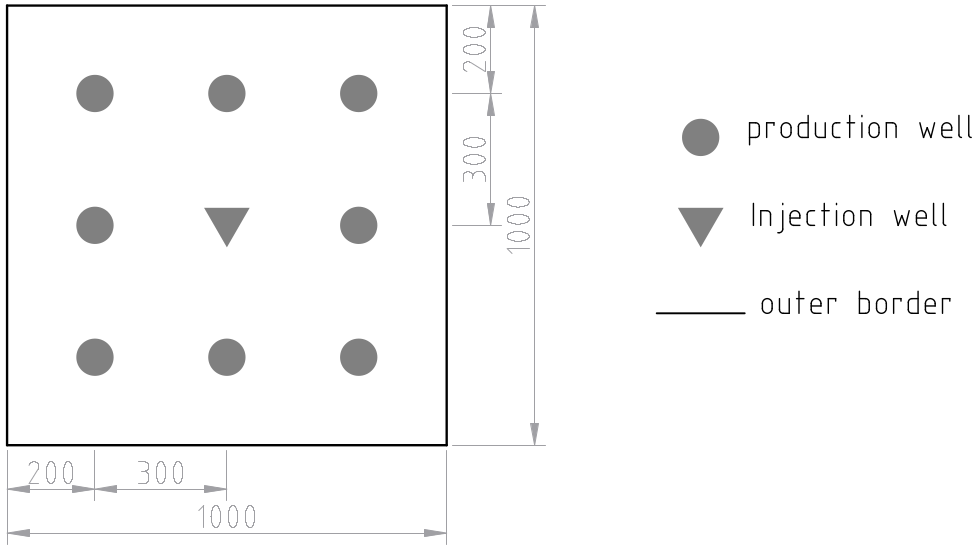
\includegraphics[height=12pc]{fig1.png}}
    \caption{Schematic representation of the computational domain.}
    \label{fig:map}
\end{figure}

The reservior contains 8 production wells and one injection well.
At the wells, the fluid flow rate was set (flow 
rates on production and injection wells). The fluid flow rate at each well was set 
as a noisy constant value. The noise
amplitude was up to $50\%$ of the average value. The time step was 1
month. The oil field development period is 30 years, the aquifer was
connected along the perimeter of the computational area. To solve
the problem of parametric identification, the development period was
divided into two intervals: the history matching interval, at which
the model parameters were adjusted, and the validation interval, at
which the forecast characteristics of the calibrated model were
evaluated. The periods were 20 and 10 years, respectively. The
amount of initial data used in the model matching on
the history matching interval is 63 pressure values randomly
selected from the entire volume of original well pressure values,
which is approximately $2.5\%$ of the available number. For the
history matching interval, 1920 values of water flow in production
wells were used. At the validation interval, the amount of original
data was 37 and 960 values for pressure and flow, respectively.

The primal and inverse problems were solved numerically using the
control volume method, the difference grid had 441 calculated nodes,
each node has its own permeability value, which is a configurable
parameter.

The history matching problem is solved for 11 variants of sets of
weight coefficients $(w_p, w_{q_w})$ used in the objective function
({\ref{mse}}). The values of the weight coefficients in the sets were
set in such a way that the condition $w_p = 1 - w_{q_w}$ was
fulfilled, where $w_{q_w}$ changed from 0 to 1 with a step of 0.1.
By changing the weight coefficients, the sensitivity of the
objective function and its gradient to different types of input data
changed. In addition, if one of the weight coefficients is equal to
0, the model is matched to only one of the two types of input data.

Research methodology: the reservoir permeability is set, the well
operation modes (fluid flow rates) are set, the primal problem is
solved, the calculated values of reservoir pressure and oil flow
rate are saved and then act as actual values. Next, a perturbation
is introduced into the original reservoir permeability, which acts as an
initial approximation in solving the inverse problem. Next, the
inverse problem is solved in order to restore such a reservoir permeability
in order to reproduce as accurately as possible the actual
values of reservoir pressure and water flow in wells, taking into
account the given weight coefficients. Further, the matched model
performs forecasting calculations, the forecast period coincides with
the validation interval, which evaluates the ability of the model to
reproduce the the development performance of interest to us, the original values of
which did not participate in the history matching process.

Figure \ref{fig:press} shows the original values of reservoir
pressure for wells at different time moments, the vertical dotted
line on this graph and on the following ones separates the intervals
of history matching and validation. Figure \ref{fig:qlic} shows the
dynamics of the total flow rate of fluid and water for production
wells, the pictograms show the original values, the lines show the
averaging of the dynamics of the corresponding indicators.
\begin{figure}
    \begin{minipage}[h]{0.48\linewidth}
      \center{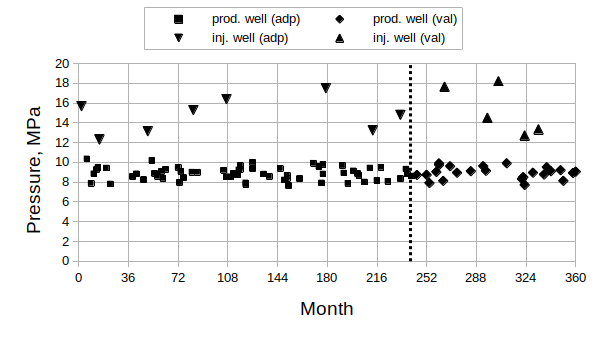
\includegraphics[height=0.60\linewidth]{fig2.png}}
\caption{Reservoir pressure values near wells used to evaluate the
accuracy of model for history matching and validation
intervals.}
      \label{fig:press}
    \end{minipage} \hfill
    \begin{minipage}[h]{0.48\linewidth}
      \center{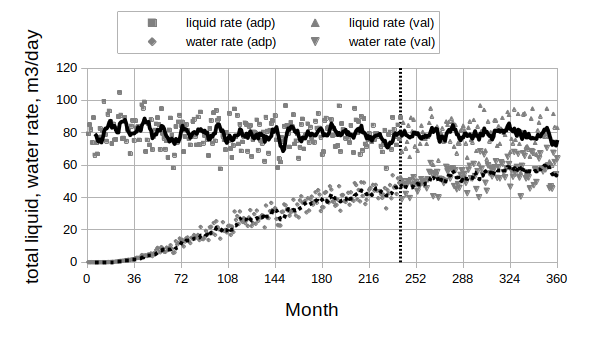
\includegraphics[height=0.60\linewidth]{fig3.png}}
\caption{The values of the total flow rates of liquid and water for
history matching and validation intervals.}
      \label{fig:qlic}
    \end{minipage}
\end{figure}
The figures show that the average values of reservoir pressure and fluid flow rate are constant throughout the simulation period, the water flow rate gradually increases as the oil is displaced by water and the front of the water saturation surge arrives at the producing wells.
The inverse problem was solved for 11 sets of weight coefficients, in which the influence of
pressure data gradually increased and the influence of water flow
decreased. Figure \ref{fig:wp} shows the values of the MAPE metrics
and the objective function $J$ for different sets of weight
coefficients. The MAPE metric is calculated for pressure indicators,
water flow rates at production wells for history matching and
validation intervals. In addition, the figure shows the MAPE metric
for permeability, which characterizes the deviation of the restored
values from the actual ones.

\begin{figure}
    \center{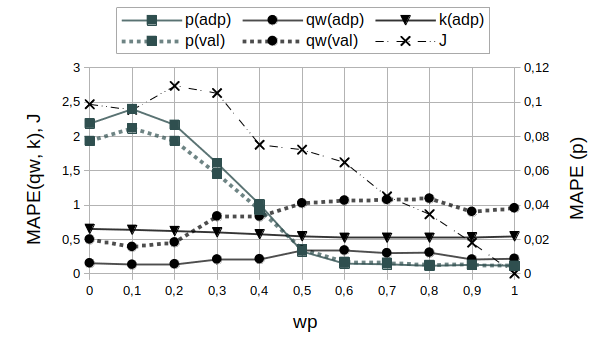
\includegraphics[height=12pc]{fig4.png}}
\caption{MAPE metric and objective function $J$ values for 11 sets
of weight coefficients for history matching
        intervals (adp) and validation intervals (val).}
    \label{fig:wp}
\end{figure}

It can be seen from the figure that, in general, the expected
inversely proportional dependence of the metric value and the
corresponding weighting coefficient is observed. Similar behavior of
the corresponding metrics for history matching and validation
intervals is also observed. However, the sensitivity of the metric
characterizing the forecast properties for the "water flow"
indicator is higher than the metric of the same indicator on the
history matching interval, which indicates the importance of
choosing one or another history matching option in terms of
forecast properties. Figure \ref{fig:wp} also shows that the
nature of the change in the objective function $J$ differs from the
nature of the change in the MAPE metric. Based on the graph, we can
conclude that when the weight coefficient $w_p$ changes in the range
from 0 to 0.3, it is most difficult for the model to satisfy the
original data. Since the main purpose of modeling is to obtain a
reliable forecast, and also taking into account the nature of the
dependence of metrics and their absolute values on weight
coefficients, it is recommended to choose the model history matching
option with the value of the weight coefficient $w_p$ = 0.1. It
should also be answered that, due to the peculiarity of the solution
of the inverse problem, none of the solutions reproduced the
original reservoir permeability, the deviation was more than 50\%,
nevertheless, the forecast characteristics of these models are
satisfactory, both for reservoir pressure and for water flow. In
practice, we do not know the real reservoir permeability, and the
solution obtained for practical problems is acceptable if it has a
satisfactory history setting and good forecast properties.

For the selected variant of the matched model and for the
limiting variants ($w_p = 0$ and $w_p = 1$), let's compare the
behavior of an additional integral indicator -- the average water
cut at the intervals of history matching and validation. The average
water cut at each point in time is calculated as $wtc =
\frac{\sum{q_w^i}}{\sum{q_l^i}}$. The average water cut of the
produced liquid is shown in Fig. \ref{fig:wtc}. Pictograms in Fig.
\ref{fig:wtc} shows water cut values for each month, lines show
averaged values for four options: the original option and 3 options
of the matched model with the weight coefficient $w_p$ equal to
0, 0.1 and 1.

\begin{figure}
    \center{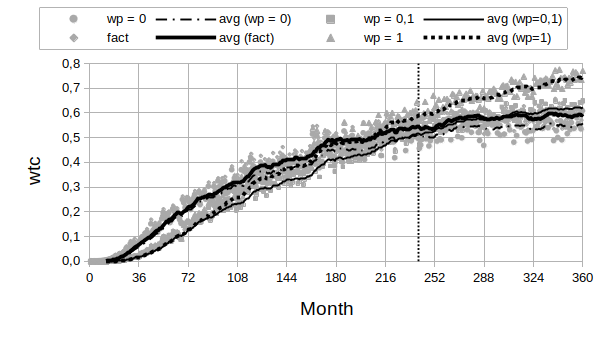
\includegraphics[height=12pc]{fig5.png}}
\caption{Produced liquid water cut (wtc) dynamics: actual values and
for 3 variants of matched model.}
    \label{fig:wtc}
\end{figure}
It can be seen from the figure that the history matching option,
taking into account only reservoir pressure $(w_p=1)$, differs
markedly from the original option both at the stage of history
matching and at the validation interval. The history matching
option, which takes into account only water flow rates $(w_p=0)$,
differs to a lesser extent from the original option, this is due to
the fact that the flow rate of phases in wells depends both directly
on the formation pressure and on the structure of fluid flows
in the interwell space, which in turn depends on reservoir pressure.
This can also be seen from the Eq. (\ref{dq_du}), where the derivative of water flow with respect to permeability depends on the derivative of pressure with respect to permeability. In terms of forecasting, the best adaptation
option is the one that comprehensively takes into account pressure and water flow, the reduced
weighting coefficient $(w_p=1)$ is explained by the fact that the
dependence on reservoir pressure, as mentioned earlier, is included
in the term of the objective function responsible for water flow and
is indirectly taken into account. Nevertheless, the presence of the 
summand responsible for reservoir pressure is important in a waterless
period of operation, when the front of the water saturation surge has
not yet reached the production wells. Thus, the use of the sum as
the objective function allows more complete use of all available
information throughout the entire modeling period.

\section{CONCLUSIONS}

As a result of the study, it was shown that the accuracy of solving
the inverse problem depends on the choice of weight coefficients
that characterize the degree of influence on the setting of a
certain type of data. The use of a combination of basic data makes
it possible to increase the degree of regularization of the problem.
The accuracy of the model for the history matching and validation
periods depends on the proportions of the weights chosen.
The dependence of the accuracy of history matching and forecasting 
for one indicator on its corresponding weighting coefficient is not linear.
The dependence is characterized by the presence of
minima and maxima, which indicates that the degree of consideration
of different indicators affect the matching process and can help to
find the most accurate solution. The feature of the methodology for solving inverse problems in the optimization formulation is minimization of a single value of the objective function, which can be a combination of elements responsible for different types of input data. It is useful to analyze other metrics that allow evaluating the accuracy of matching and forecasting when solving inverse problems.
Given the availability of a set of calibrated models,
third-party metrics will allow you to choose the most appropriate
model in terms of the requirements for it.

\section{FUNDING}
The research was carried out within the  state assignment of
Ministry of Science and Higher Education of the Russian Federation
(project no. 121030500156-6).

\begin{thebibliography}{20}


\bibitem{mus} E. N. Musakaev, S. P. Rodionov, D. Y. Legostaev, and V. P. Kosyakov,
 "Parameter identification for sector filtration model of an oil reservoir with complex structure",
 AIP Conference Proceedings 2125, 030113 (2019).

\bibitem{kos} V. P. Kosyakov, "Structural and Parametric Identification
of an Aquifer Model for an Oil Reservoir". Lobachevskii J. Math.
{\bf 41}, 1242--1247 (2020).

\bibitem{bas} K. S. Basniev, N. M. Dmitriev, R. D. Kanevskaya, and V. M. Maksimov,
\textit{Underground hydromechanics}. M.-Izhevsk: Institute for
Computer Research, 2006 [in Russian].

\bibitem{azi} H. Aziz and E. Settari, \textit{Mathematical modeling of reservoir systems}.
 M.-Izhevsk: Institute for Computer Research, 2004 [in Russian].

\bibitem{opt} V. P. Kosyakov and S. P. Rodionov, "Optimal control of wells on the basis
of two-phase filtration equations", Proceedings of MIPT {\bf 8} (3),
79--90 (2016).

\bibitem{leg} V. P. Kosyakov and  D. Yu. Legostaev, "Using elements of machine learning to
solve the inverse problem of reconstructing the hydraulic 
conductivity feld for a fltration problem", Tyumen State University
Herald. Physical and Mathematical Modeling. Oil, Gas, Energy {\bf 8}
(2 (30)), 129--149.

\end{thebibliography}

\end{document}
